\documentclass[]{article}
%opening
\title{Writeup Document}
\author{Alex Miller}
\addtolength{\oddsidemargin}{-.875in}
\addtolength{\evensidemargin}{-.875in}
\addtolength{\textwidth}{1.75in}
\addtolength{\topmargin}{-.875in}
\addtolength{\textheight}{1.75in}
\setcounter{secnumdepth}{0}
\usepackage{cancel}
\usepackage{amssymb}
\usepackage{amsmath}
\usepackage{hyperref}
\usepackage{graphicx}
\graphicspath{ {./} }
\usepackage[ruled,vlined, linesnumbered]{algorithm2e}
\DontPrintSemicolon


\begin{document}
\maketitle

\section{Changes}
\subsection{Changes to the design}
I have made the following addresses changes to my project's design, broken down by module:
\begin{itemize}
	\item Top level modules (serial.c and parallel.c)
	\begin{itemize}
		\item I modified serial.c and parallel.c to take in an optional flag denoting that the programs should be run in "correctness testing" mode. In this mode, $chksum\_serial()$ and $chksum\_parllalel()$ would not dispatch packets from $n$ sources for $M$ seconds, but $n * M$ packets total. The values these functions would return (with this flag specified) would not be throughput numbers but amalgamated checksums, as described in assignment 2.
	\end{itemize}
	\item Algorithm implementation level (chksum.c)
	\begin{itemize}
		\item I modified both  $chksum\_serial()$ and $chksum\_parallel()$ to take in the additional flag denoting whether they should generate checksums in correctness testing mode or not.
		\\\\
		If so, the dispatchers for these functions would not rely on a timed approach to halting packet generation, but would instead halt themselves and their threads after generating $M * n$ packets. The long integer returned by these methods would not represent their respective throughputs, but amalgamated checksums.
		\\\\
		Threads launched by the parallel dispatcher would not tally throughput for queues but amalgamated checksums instead. This requires the definition of the following worker methods:
		\begin{itemize}
			\item $void$ $*L\_worker\_test(void$ $*args)$
			\item $void$ $*H\_worker\_test(void$ $*args)$ 
			\item $void$ $*A\_worker\_test(void$ $*args)$
		\end{itemize}
		all of which would implement the behaviors of their namesakes, but instead record amalgamated checksums and not mere throughput. These methods would deviate from their original versions in that they generate amalgamated checksums and only exit once all queues are empty and the closing of the system is signaled. However, the $A\_worker\_test()$ method has the problem that it can't necessarily tell when \textit{all} queues are empty. As such, when indicated, $clear\_queue$ (discussed below) will be responsible for generating returning the amalgamated checksum of any packets left in a queue upon cleanup, and adding that checksum to $chksum\_parallel()$'s return value. This will insure that, if $A\_worker\_test$ isn't able to reach all packets enqueued by the dispatcher, that it at least generated the correct checksums for all packets it was able to reach.
		\\\\
		$chksum\_parallel()$ would be responsible for setting $worker\_method$ to one of these functions when specified by the correctness testing flag.
		\item My original design for both the serial and parallel dispatchers utilized a scheme in which each would repeatedly calculate and check whether they had surpassed the allotted time limit. Once written, however, this method seemed bulky and to incur no small amount of increased overhead and complexity within the packet dispatching loops.
		\\
		Now, rather than having the dispatching threads calculate time intervals themselves, they both call the new method $start\_timed\_flag()$, which takes in two arguments:
		\begin{itemize}
			\item volatile bool *done : a volatile pointer to a malloced flag
			\item int M : a integer specifying a number of milliseconds
		\end{itemize}
		This method spawns a new thread that sleeps for $M$ milliseconds before setting the value pointed to by $done$ to $true$. The method than detaches the spawned thread and returns.
		\\
		Dispatching sections can then just operate so long as the value pointed to by $done$ is $false$. In $chksum\_serial()$, this value is allocated before the test is run. In $chksum\_parallel$, this value is allocated in the $create\_queue\_pool()$ method and pointed to by all $packet\_queue\_t$ instances in the queue pool.
		\\
		This method does incur the extra overhead of managing an additional thread, which may complicate performance analysis. However, as that thread's primary task is sleeping, the effect should be negligible.
		\item I also steamlined the behavior defined by the Awesome load balancing strategy:
		\begin{itemize}
			\item Within an infinite while loop, the thread attempts to acquire a queue's associated lock with it's $trylock()$ method.
			\item If it succeeds, the thread waits to enter the critical section:
			\begin{itemize}
				\item The thread attempts to dequeue from the queue and binds the result to a pointer called $packet$.
				\item The thread then unlocks the queue's lock
				\item If $packet \neq NULL$, then the thread generates a checksum for the packet and frees it.
				\item At this point, if the thread has been signaled to close, it returns
				\item Otherwise, it atomically increments the queue's $through\_count$ counter
			\end{itemize}
			\item Once it has either attempted to acquire the lock and failed or has exited the critical section, the thread checks if it has been signalled to close. If it has it returns. Otherwise, the thread moves onto the next queue.
		\end{itemize}
	\end{itemize}
	\item Queue data structure (queue.c)
	\begin{itemize}
		\item My original declaration of my queue-pool initialization method was as follows:
		\\\\
		\textit{packet\_queue\_t *create\_queue\_pool(int num\_q, int D, char L) : allocate an array of $num\_q$ packet\_queue\_t structs, each of depth $D$. Each queue should have a lock of type $L$ associated with it. If $L$ does not specify a char code for a valid lock (if L is not t, p, m, or a), then no locks are allocated.}
		\\\\
		This method is now declared as:
		\\\\
		packet\_queue\_t *create\_queue\_pool(int num\_q, int D, char L, int n) : allocate an array of $num\_q$ packet\_queue\_t structs, each of depth $D$. Each queue should have a lock of type $L$ associated with it. If $L$ does not specify a char code for a valid lock (if L is not t, p, m, or a), then no locks are allocated. Each lock in the queue pool will be initialized to work with $n$ total threads.
		\item My implementation also now includes the method:
		\\\\
		long clear\_queue(packet\_queue\_t *Q, bool correct) 
		\\\\
		This method frees any packets in a queue -- it is used to cleanup allocated system resources. If $correct = true$, then it also generate an amalgamated checksum for the packets left in a queue and returns this value. Otherwise it merely returns $0$ 
	\end{itemize}
	\item Lock data structure (lock.c)
	\begin{itemize}
		\item No changes to report
	\end{itemize}
	\item Testing script (test\_script.sh)
	\begin{itemize}
		\item I neglected to state that I would vary trial numbers based on the type of packet generator specified by an experiment. Trials using a uniform packet generator will still utilize 5 trials. Trials using an exponential packet generator, however, will utilize 11 trials.
		\item Additionally, I will include another file, $correct\_test\_script.sh$, which utilizes the optional correctness testing scheme I described above. This script will verify that amalgamated checksums are consistent across $chksum\_serial()$ and $chksum\_parallel()$, for all load balancing strategies.
		\item Finally, I also want to test my Awesome load balancing on Uniform packets. I will therefore redo Experiment 2: Speedup with Uniform Load, but instead of using the HomeQueue strategy I will use my new Awesome strategy, in addition to my other tests. 
	\end{itemize}
	\item These changes are consistent with my previously stated invariants
\end{itemize}

\subsection{Changes to Test plan:}
As mentioned above, I will not try to verify if my Awesome load balancing strategy is strictly consistent with my serial implementation. As the Awesome strategy doesn't map worker threads to queue, the possibility remains that the threads exit our correctness testing implementation prior to generating checksums for all generated packets. As such, worker threads themselves might not generate an amalgamated checksum that is consistent $chksum\_serial()$. This discrepancy is mitigated by the use of $clear\_queue()$. For now, I am deeming this a sufficient test of correctness for my Awesome load balancing strategy. To desire more would mean having to alter the structure of the strategy as to make it a non-meaningful test of correctness.
\section{Results}
As of writing this, $correct\_test\_script.sh$ confirms that my implementations are consistent. Moreover, testing revealed that while timing my implementation using the StopWatch\_t type was inconsistent, my timed flag implementation was consistent; For M = 2000 ms, test\_script.sh should complete after ~80 minutes. When using stopwatch based dispatchers, the script did not complete its task within 90 minutes; when using my timed flag, the test script completed its run in at most 82 minutes.
\\\\
The raw performance data for the Idle Lock Overhead and Speedup tests are stored in a folder called $HW3b/hw3b/exp\_data$. This folder contains the .csv files that describe performance data for a given experiment. overhead.csv describes the data from experiment 1. speedup.csv contains all other necessary data
\\
This data was collected by running implementations for given number of trials, calculating measurements per trial, and taking median values. As such there is no other collected data other than median speedup and throughput. That data was not recorded as it did not serve the purpose of analysis and would've have complicated my data storage scheme.
\\\\
As per how many trials I utilized; for experiments utilizing uniform packets, I used 5 trials; for experiments utilizing exponential packets, I used 11 trials.
\\\\
I took this data and plotted it using the script analyze.py. These graphs are stored in the folder $HW3b/Docs/graphs$. I will display these graphs below:
\subsection{Experiment 1: Idle Lock Overhead}
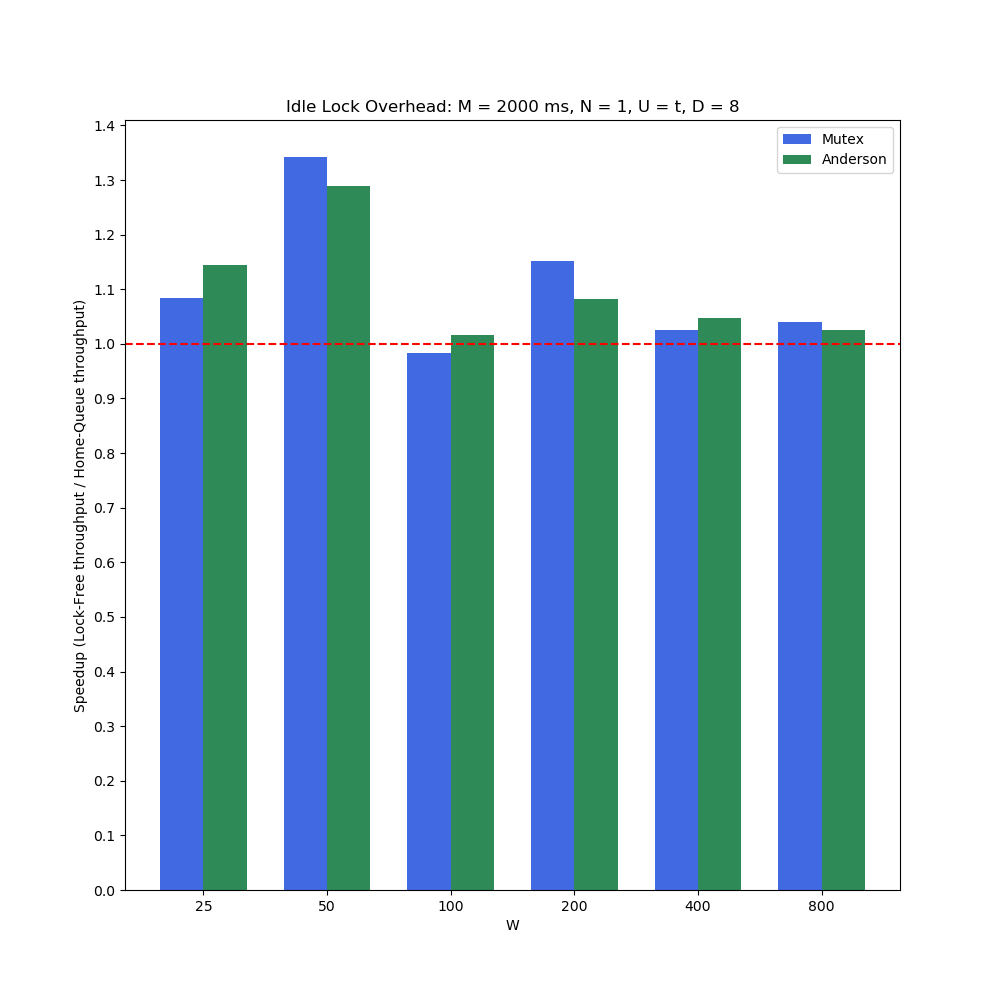
\includegraphics[scale=0.5]{graphs/overhead.png}\\
\subsection{Experiment 2: Speedup with Uniform Load}
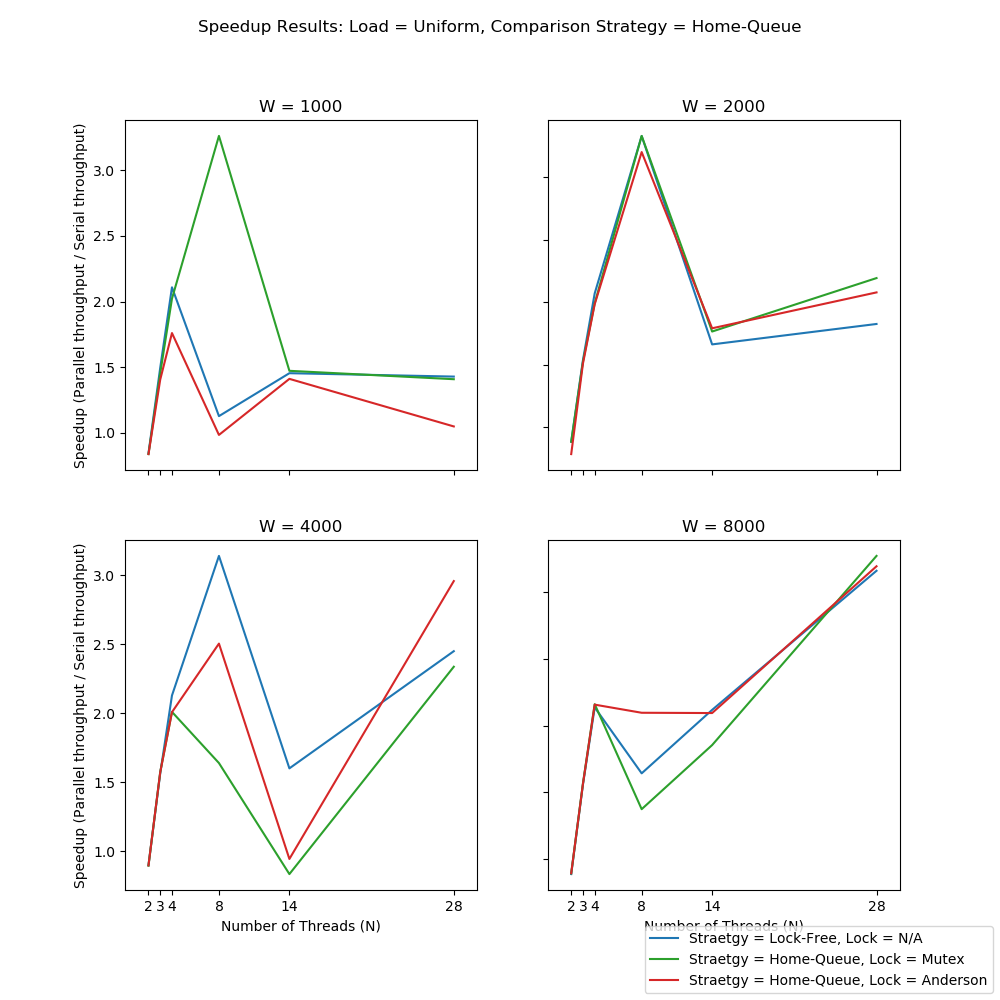
\includegraphics[scale=0.5]{graphs/speedup_t:H.png}\\
\subsection{Experiment 3: Speedup with Exponential Load}
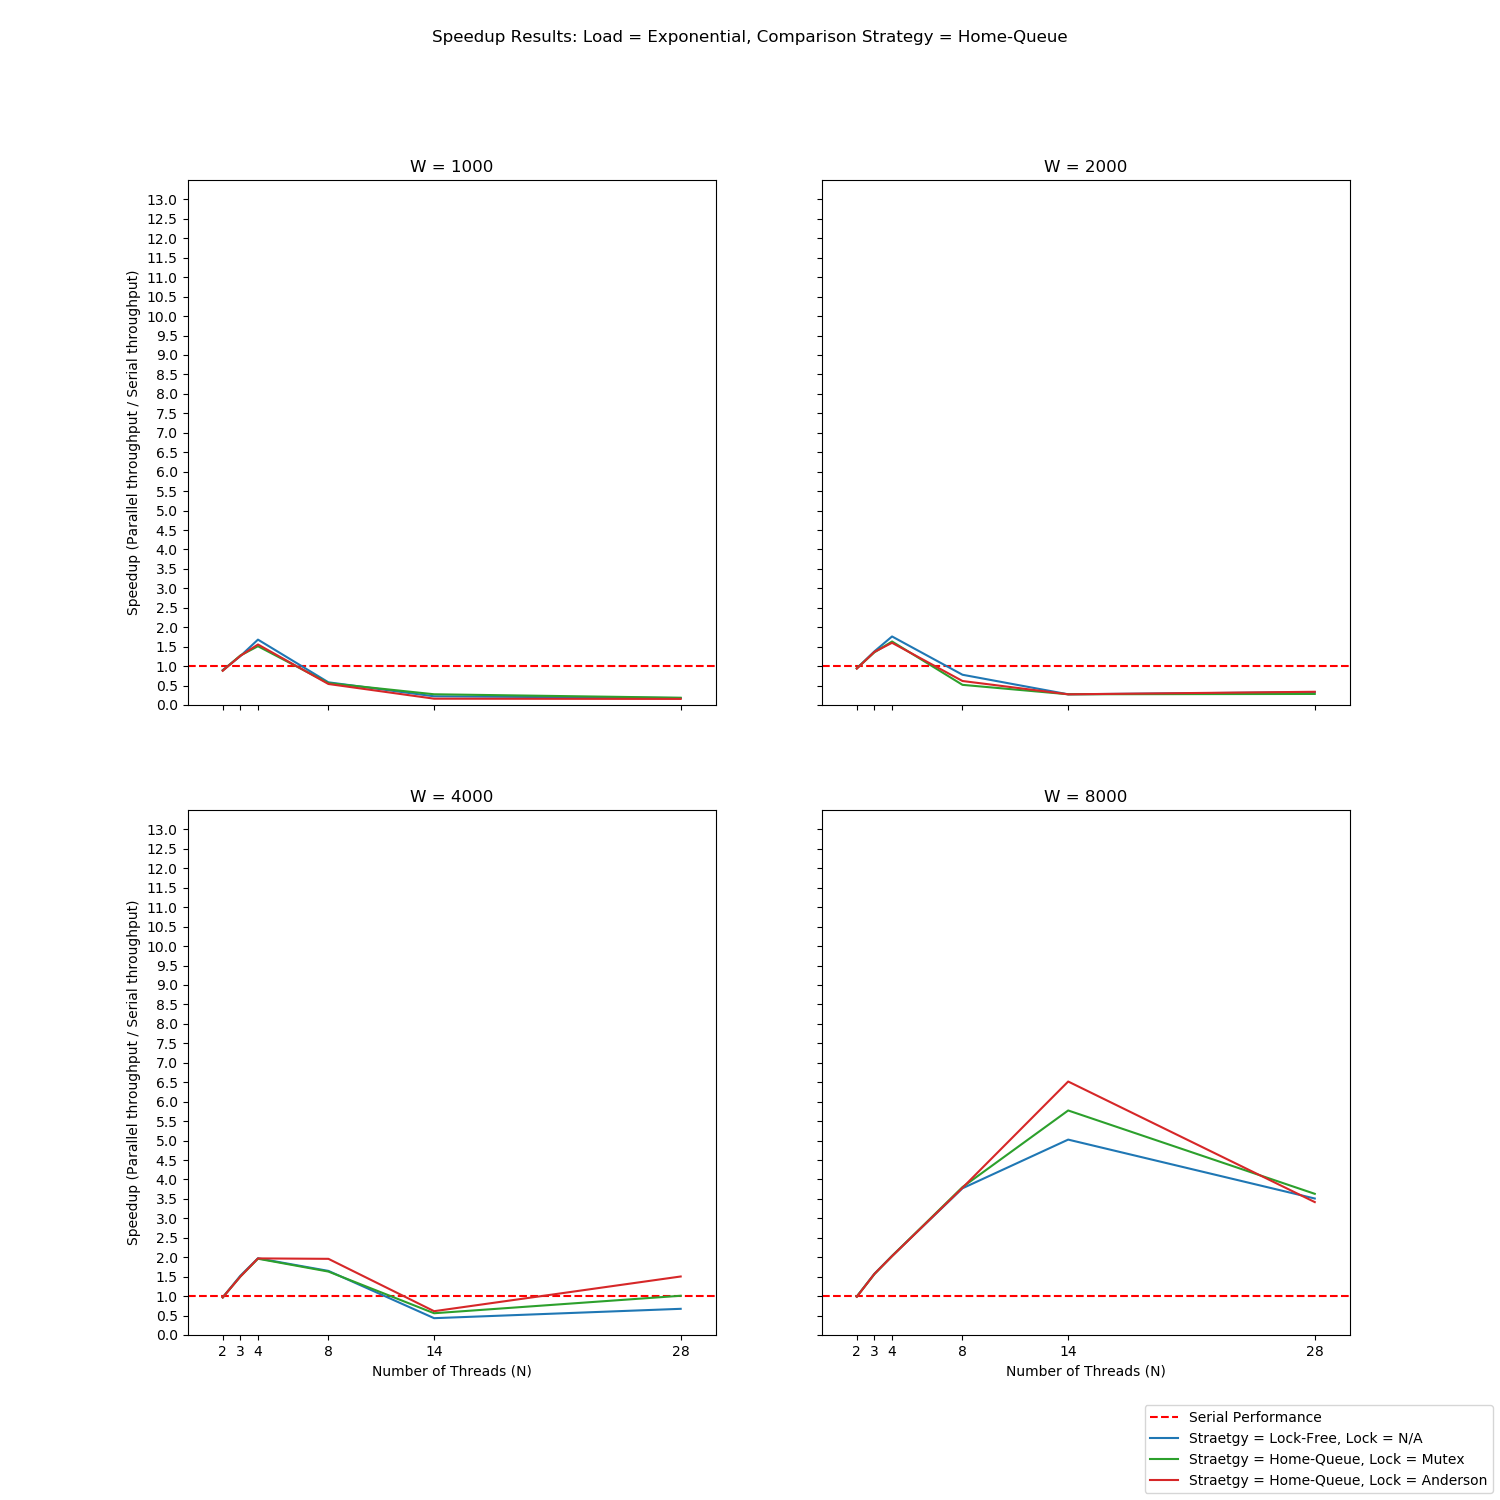
\includegraphics[scale=0.5]{graphs/speedup_f:H.png}\\
\subsection{Experiment 4: Speedup with Exponential Load (Awesome Test)}
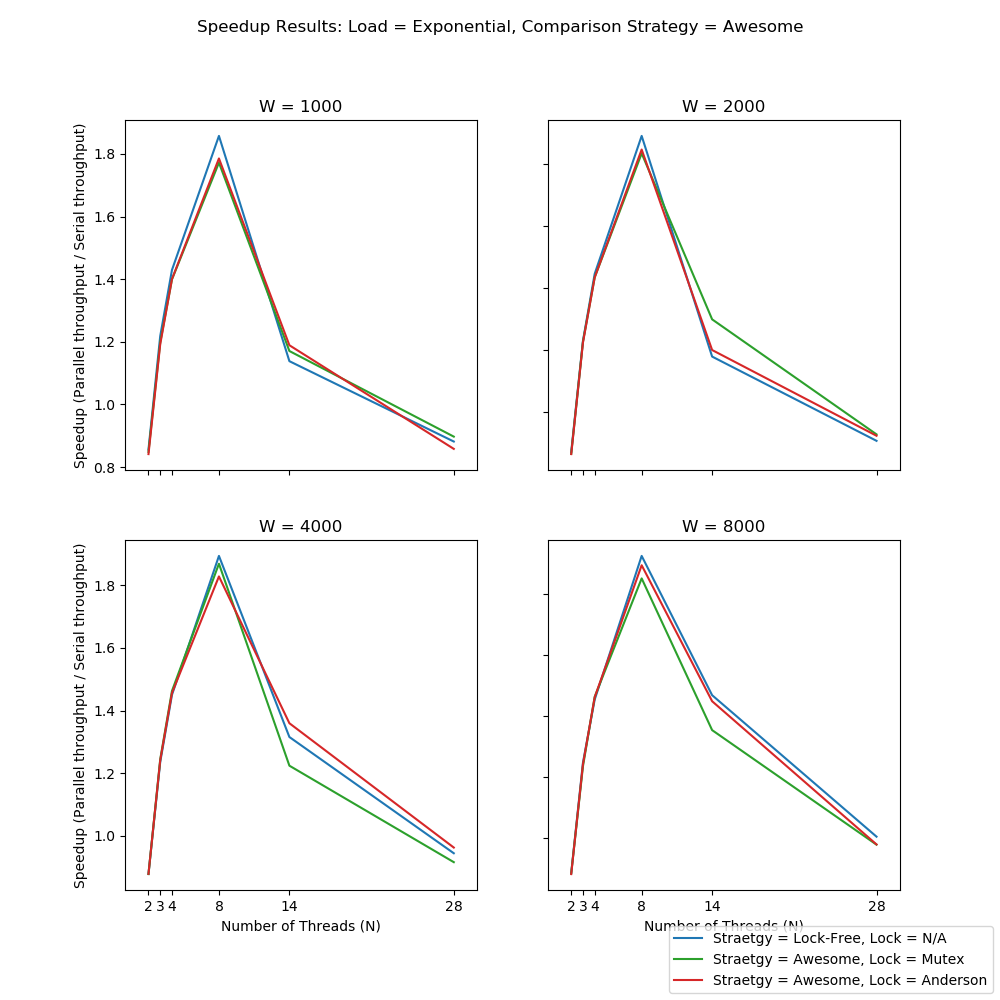
\includegraphics[scale=0.5]{graphs/speedup_f:A.png}\\

\section{Analysis}

\subsection{Idle Lock Overhead:}
\textbf{Hypothesis:}
The purpose of this test is to measure the overhead of using locks in the HomeQueue strategy in comparison to the LockFree strategy. Between these two strategies, I expected the HomeQueue strategy to entail greater overhead in its use of a lock around the worker thread's invocation of $dequeue()$. This hypothesis followed from  observations in HW3a -- in counter tests, for $n = 1$, both the Mutex lock and Anderson's lock displayed 10x slowdown over ideal, LockFree performance. Therefore, I expected to see similar, observable, levels of overhead in these tests. At the very least, I ruled out the possibility of any observed speedup of HomeQueue over LockFree. 
\\
For larger values of $W$, I expected the relative overhead of HomeQueue over LockFree to decrease. This follows from our observations in HW2 -- larger values of $W$ entailed longer packet processing times, which gave more opportunities for parallelism and speedup. In this case, larger values of $W$ will otherwise outweigh the increased overhead entailed in acquiring locks, reducing the relative overhead of HomeQueue over LockFree.
\\
As to the relative performance of these tests across the use of our different locks: both the Mutex and our Anderson locks showed similar performance for use with a single acquiring thread -- as demonstrated in HW3a, the Anderson Lock entailed a 10.33x slowdown when used with a counter, while the Mutex lock performed similarly with a 10.60x slowdown. Therefore I expected similar Idle Lock Overhead from our uses of these locks in this experiment.
\\\\
\textbf{Result analysis and discussion:}
As the data demonstrates, these expectations were not accurate. For one, it is not entirely clear from the data that the use of locks in the HomeQueue strategy entailed any non-trivial amount of overhead -- in some cases the data suggests that the HomeQueue strategy allowed for small levels of speedup. Notably, where I predicted to observe the most relative slowdown of HomeQueue over LockFree, namely $W = 25$,  both HomeQueue tests actually performed better relative to their corresponding LockFree test than any other data point. Both tests actually experienced speedup over LockFree, with the Mutex lock test processing 3.5\% and the Anderson lcok test processing 7.9\% more packets than their corresponding LockFree test. Overall, out of 12 total data points, 7 demonstrated relative speedup of our HomeQueue implementation over our LockFree implementation.
\\
This result may be explained or otherwise better understood through a comparison of the contexts in which these locks were tested for overhead between HW3a and HW3b. In 3a, these locks were tested by setting them around a single volatile counter increment (with accompanying bounds check). However, in my HomeQueue implementation, they are set around a while loop based on my dequeue() method, which includes a two volatile reads, a modulo operation, as well as a volatile increment. Additionally, both my LockFree and HomeQueue implementations must perform the necessary packet processing.
\\
This discrepancy may go far to explain we don't see something close to 10x slowdown of HomeQueue over LockFree. As the critical section around which the locks are placed is significantly larger here than in our counter tests, it makes sense that the effect of overhead in their use should be less significant or otherwise observable. Moreover, as threads under either load balancing strategy also have to process the packets they dequeue, the time spent locking and unlocking while using the HomeQueue strategy is further overshadowed by thread operations outside the critical section.
\\
As such, we can understand our results as not demonstrating inherent speedup in our use of locks, but rather a principle that was somewhat gleaned in my results from HW3a -- critical section size can otherwise mitigate the overhead experienced in using locks.
\\\\
This explanation also works to explain why we should not see decreasing relative slowdown of HomeQueue over LockFree for increasing values of $W$. Increasing $W$ implies that packets, on average, take longer to process. HomeQueue tests utilizing larger values of $W$ should therefore, in theory, experience less slowdown in comparison to their corresponding LockFree. That we don't see this relationship reflected in the data is therefore confusing. Rather, as noted above, we see relative speedup of HomeQueue (using either lock) over LockFree for some smaller values of $W$, such as $W = 25$, while we see slowdown for larger values, such as $W = 100$ -- in that case, Mutex and Anderson tests processed 4.11\% and 4.49\% less packets than the corresponding Lock Free test.
\\
However, we may apply similar reasoning from our prior observations here to understand this complication. That relative overhead of HomeQueue over LockFree does not necessarily decrease for larger values of $W$ could be explained by the fact that, even when using $W = 25$, the overhead of dequeueing packets was already sufficient to overshadow the overhead entailed with the use of locks. 
\\\\
The data, therefore, suggests the following analysis: the use of locks do indeed entail the presence of overhead -- it is not wrong to think that HomeQueue is a more expensive implementation than LockFree. However, at least when only using one worker thread, the Anderson and Mutex locks are able to perform well enough for this application such that their inclusion is otherwise negligible in considering program performance. That we see variations in the data is then explained by other runtime abberations that the system the implementations were tested on encountered -- this is further supported by the fact that only one HomeQueue trial ($W = 25, Lock = Anderson$) displayed performance that varied from its LockFree comparison by more than 5\%.
\\\\
As to the relative performance of the Mutex and Anderson locks: as expected both locks displayed similar performance. Both locks outperformed the other in an (about) equal number of tests -- the Mutex lock decisively displayed less overhead in 2 out of 6 tests, and the Anderson lock 3 out 6 (we take decisive to mean that one test outperformed the other by a margin greater than 1.0\%). The difference in either locks' cumulative throughput is also negligible; tests using the Anderson lock only processed 3.4\% more packets than Mutex tests.
\subsection{Speedup with Uniform Load:}
\textbf{Hypothesis:}
The purpose of this test is to asses the performance of our LockFree and HomeQueue implementations in relation to our serial implementation under a uniform packet distribution. As larger values of $W$ imply more opportunity to parallelize the computation of checksums, I expected both parallel implementations to perform better as $W$ increased. Therefore, while using both our LockFree and HomeQueue strategies,  I  expected increased speedup of parallel.c over serial.c for greater values of $W$. 
\\
The same might be said for larger values of $n$ given a fixed value for $W$ -- for one, larger $n$ implies that implementations use more sources and have to process more packets, leaving room for parallelization. Additionally, a greater number of worker threads might be able to work together more efficiently than a single thread. However, larger values of $n$ also imply larger amounts of overhead in managing threads and queues. There is also the concern that once $n >$ the number of cores in the system (14) should entail loss in performance -- as observed in HW2.
\\
Therefore, in comparing the observed speedup for different values of $W$, among all load balancing strategies, I expected to see increased speedup over our serial implementation for larger values of $W$. For a given value of $W$, I expected to see greater speedup for greater values of $n$ -- as observed in the results for HW2, I expected speedup to appear linear for large enough values of $W$ and $n \leq 13$. However, I expected this to be accompanied by diminishing returns on speedup for larger values of $n$, especially $n > 13$.
\\
Between load balancing strategies, I expected to see consistently faster performance from LockFree, as opposed to HomeQueue, due to the overhead entailed in using locks. Between the use of Mutex and Anderson's locks, I expected to see similar levels of performance -- in line with our hypothesis from Experiment 1. Moreover, I did not expect to see discrepancy in lock overhead for varying values of $n$, as all locks used in my Home Queue implementation are uncontested.%Maybe discuss convergence of performance to LockFree for succificiently large W%
\\\\
\textbf{Result analysis and discussion:}


\subsection{Speedup with Exponential Load:}
\textbf{Hypothesis:}
I adopt the same reasoning from the prior experiment. However, because this test employs a exponential packet generator, the amount of work each thread must perform is constantly increasing at an exponential rate. This may make it seem like we should experience even greater opportunities for speedup even as we continue to process packets. However, as different sources generate packets with different curves that describe the work needed to generate a checksum for the $i$-th packet, all of which merely share an average amount of work, this leaves the possibility of some queues becoming overburdened with large packets as the test goes on, creating performance bottlenecks. Therefore, while greater values of $W$ should entail greater opportunities for speedup, without load balancing, this effect will not be as noticeable as when using an Uniform packet generator.
\\
Like the previous experiment, in comparing the observed speedup of our parallel implementations over our serial implementation for different values of $W$, I expected increased speedup for larger values of $W$. For a given value of $W$, I expected to see greater speedup for greater values of $n$ -- as observed in the results for HW2, we can expect speedup to appear linear for large enough values of $W$ and $n \leq 13$. However, this is accompanied by diminishing returns on speedup for larger values of $n$, especially $n > 13$.
\\
Between load balancing strategies, I expected to see consistently faster performance from LockFree, as opposed to HomeQueue, due to the overhead entailed in using locks. Between the use of Mutex and Anderson's locks, I expected to see similar levels of performance -- in line with our hypothesis from Experiment 1. Moreover, I did not expect to see discrepancy in lock overhead for varying values of $n$, as all locks used in my Home Queue implementation are uncontested. %Maybe discuss convergence of performance to LockFree for succificiently large W%
\\\\
\textbf{Result analysis and discussion:}

\subsection{Speedup with Exponential Load (Awesome Test)}
For my final experiment, I proposed to redo the prior experiment but using $S \in \{LockFree, Awesome\}$.
\\\\
\textbf{Hypothesis:} Like the previous experiment, in comparing the observed speedup of our parallel implementations for different values of $W$, I expected increased speedup for larger values of $W$. For a given value of $W$, I expected to see greater speedup for greater values of $n$ -- as observed in the results for HW2, we can expect speedup to appear linear for large enough values of $W$ and $n \leq 13$. However, this is accompanied by diminishing returns on speedup for larger values of $n$, especially $n > 13$. I expected this estimation to be true for both our LockFree and Awesome load balancing strategies.
\\
Unlike the previous experiment, while the speedup of our LockFree implementation will suffer due to the use of an exponential packet generator, I expected that the speedup of our Awesome implementation  would not. Rather, because worker threads are able to search for work to do, I expected that they would alleviate uneven burdens put on the implementation's various queues due to the exponential distribution. This is the situation under which the Awesome strategy should succeed; otherwise, if there was an even distribution of work among queues, there would be no performance to be gained from making threads search for work. In this test then, I expected that the Awesome strategy would outperform the LockFree strategy for all values of $n$ and $W$.
\\
However, I also expected that this increase in performance from load balancing would be mitigated -- under Awesome strategy, the queues' locks can be in contention among different worker threads, making them a greater source of slowdown than they were when used in the HomeQueue strategy. Performance between the two locks, however, should be similar, if not with the Mutex lock performing a bit better -- this is confirmed by our curves from HW3a, Experiment 2. This experiment demonstrated that the Mutex lock consistently outperforms our Anderson lock in the presence of contention -- which is bound to occur under the Awesome strategy.
\\\\
\textbf{Result analysis and discussion:}

	
\end{document}
